% \documentclass[handout,aspectratio=169,11pt]{beamer}
\documentclass[aspectratio=169,11pt]{beamer}

\usepackage[T1]{fontenc}
\usepackage[utf8]{inputenc}
\usepackage[english]{babel}
\usepackage{animate}
\usepackage{csquotes}
\usepackage{lmodern}
\usepackage{amsmath,amssymb}
\usepackage{cancel}
\usepackage{tikz}
\usepackage{fontawesome5}
\usepackage{verbatim}
\usepackage{pgfplots}
\usepackage{booktabs}
\pgfplotsset{compat=1.18}
\usepackage{subcaption}
\usetikzlibrary{decorations.pathreplacing, positioning}
\usepackage{listings}
\usepackage{hyperref}
\usepackage[backend=biber,style=authoryear]{biblatex}
\addbibresource{references.bib}

\usetheme{Warsaw}
\usecolortheme{wolverine}
\usefonttheme{serif}
\useinnertheme{circles}
\useoutertheme{shadow}

\hypersetup{
  colorlinks=true,
  linkcolor=black,
  filecolor=cyan,
  citecolor=gray,    
  urlcolor=magenta,
  pdftitle={Introduction to Finite Difference Methods},
}

\setbeamertemplate{footline}[frame number]
% \setbeameroption{show notes} # <--- Comment this out to hide the notes
\setbeamertemplate{note page}[plain]
\setbeamertemplate{navigation symbols}{} % remove navigation symbols
\setbeamercovered{transparent} % make covered text transparent
\setbeamertemplate{headline}{}

\lstdefinestyle{pythoncompact}{
  language=Python,
  basicstyle=\ttfamily\footnotesize,
  keywordstyle=\color{blue!70!black}\bfseries,
  commentstyle=\color{green!50!black}\itshape,
  stringstyle=\color{red!70!black},
  showstringspaces=false,
  breaklines=true,
  tabsize=2,
  columns=fullflexible,
}

\title{An Introduction to Finite Difference Methods}
\subtitle{A Tour Through Partial Differential Equations}
\author{Manuel A. Diaz}
\institute{InspiraSTEM Internship}
\date{\today}
\titlegraphic{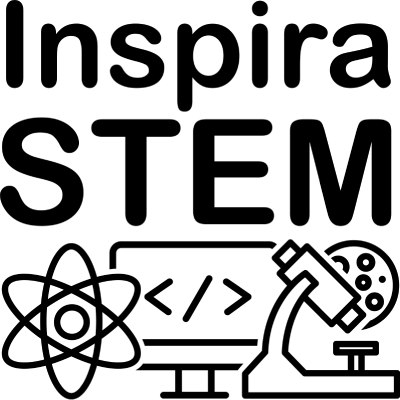
\includegraphics[height=1.35cm]{figures/InspiraSTEM_logo.png}}

% \AtBeginSection[]{
%   \begin{frame}{Outline}
%     \tableofcontents[currentsection]
%   \end{frame}
% }

%%%%%%%%%%%%%%%%%%%
% Begin document
%%%%%%%%%%%%%%%%%%%
\begin{document}

\begin{frame}
  \titlepage
\end{frame}

\begin{frame}{Outline}
  \tableofcontents
\end{frame}

\section{Motivation}

\begin{table}[ht]
\centering
%\caption{Taylor Table}
\begin{tabular}{lcccc}
\toprule
 & $f_j$ & $f'_j$ & $f''_j$ & $f'''_j$ \\
\midrule
$f'_j$ & \color{red}$0$ & \color{red}$1$ & \color{red}$0$ & \color{gray}$0$ \\
\midrule
$a_0f_j$ &
\color{blue}$a_0$ &
\color{blue}$0$ &
\color{blue}$0$ &
\color{gray}$0$ \\
\midrule
$a_1f_{j+1}$ &
\color{blue}$a_1$ &
\color{blue}$a_1h$ &
\color{blue}$a_1\dfrac{h^2}{2}$ &
\color{gray}$a_1\dfrac{h^3}{6}$ \\
\midrule
$a_2f_{j+2}$ &
\color{blue}$a_2$ &
\color{blue}$2ha_2$ &
\color{blue}$a_2\dfrac{(2h)^2}{2}$ &
\color{gray}$a_2\dfrac{(2h)^3}{6}$ \\
\bottomrule
\end{tabular}
\end{table}

$$f_{j{\color{red}\pm}1}=f_j{\color{red}\pm} hf_j'+\frac{h^2}{2}f_j''{\color{red}\pm}\frac{h^3}{6}f_j'''+\cdots$$

$$f_j = {\color{orange}a_0} f_{j} + {\color{orange}a_1} f_{j+1} + {\color{orange}a_2} f_{j+2}$$


\begin{frame}[allowframebreaks]{References}
  \printbibliography[heading=none]
\end{frame}

\end{document}
